\subsection{Kennzahlen}
    Auch in diesem Fallbeispiel wurde eine Reihe an Kennzahlen ermittelt,
    die in diesem Kapitel präsentiert werden.

    \paragraph*{Struktur eines Graphen}
    Zum Verständnis der Zahlen trägt Abbildung \ref{image:findingNewsFiguresDbModel} bei,
    welche den Aufbau des Graphen visualisiert.
    Wegen der beschriebenen Überschneidung mit dem ersten Fallbeispiel,
    sind die übereinstimmenden Knoten hier nicht nochmals dargestellt.
    Wie im vorherigen Beispiel wird außerdem auf die Darstellung von
    Referenzen verzichtet.

    \begin{figure}[htb]
        \centering
        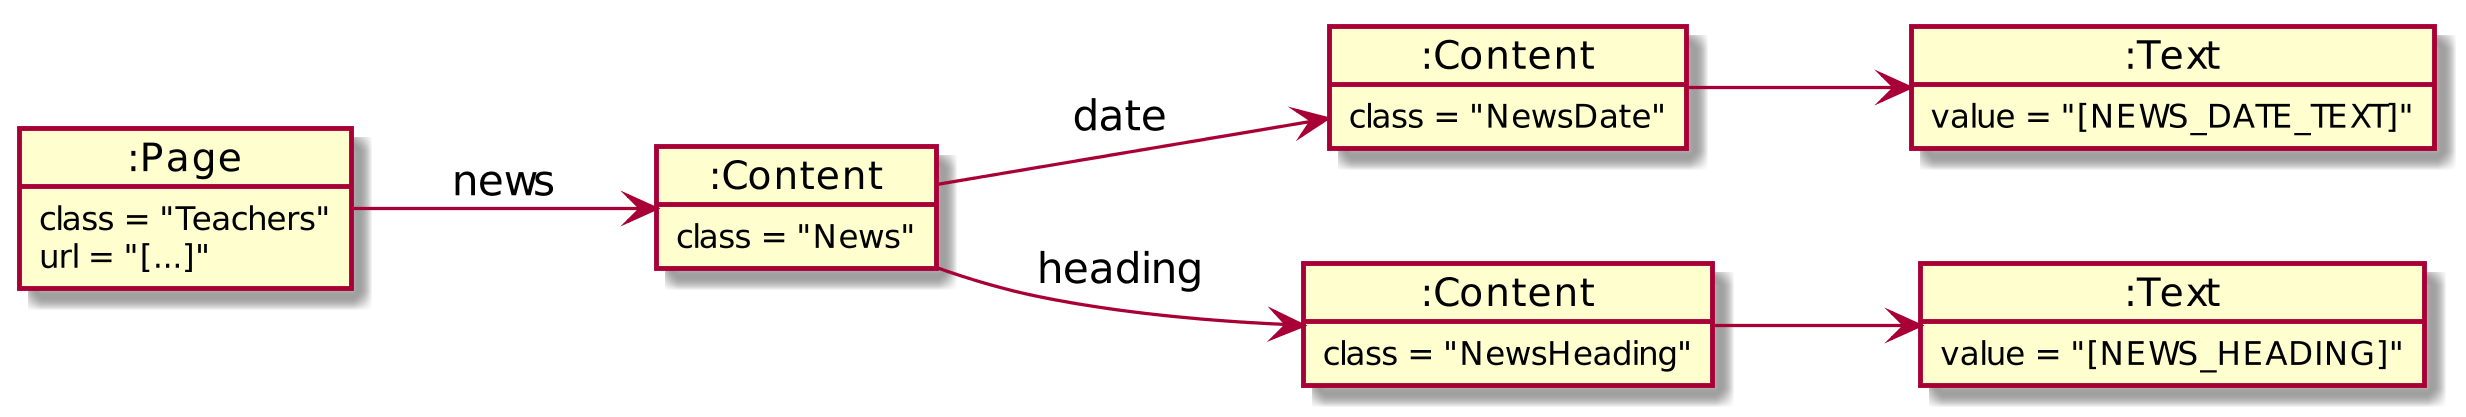
\includegraphics[scale=\imageScalingFactor]{../resources/findings/case-study-2/dbmodel.png}
        \caption{Die Struktur des Graphen einer Webseite über aktuelle Meldungen}
        \label{image:findingNewsFiguresDbModel}
    \end{figure}

    \paragraph*{Präsentation der Kennzahlen}
    Die Tabellen in Anhang \ref{section:appendixExample2Figures} präsentieren die gesammelten Kennzahlen.
    Die Gruppierung der Knoten nach ihren Labels ist in Tabelle
    \ref{table:findingsNewsFiguresNodesByLabel} zu sehen.
    Die Häufigkeit der Inhaltsklassen stellt Tabelle
    \ref{table:findingsNewsFiguresContentNodesByClass} dar.
    Tabelle \ref{table:findingNewsFiguresEdgesByLabel} gruppiert die Kanten der Datenbank
    nach ihren Labels und Tabelle
    \ref{table:findingsNewsFiguresEdgesByStartEndNodeLabel}
    stellt heraus, welche Knotenarten diese Kanten verbinden.
    Zuletzt betrachtet Tabelle \ref{table:findingsNewsFiguresSharedNodes}
    die Frage, welche Knoten mehrfach referenziert wurden.
